\begin{figure}[t]
\centering
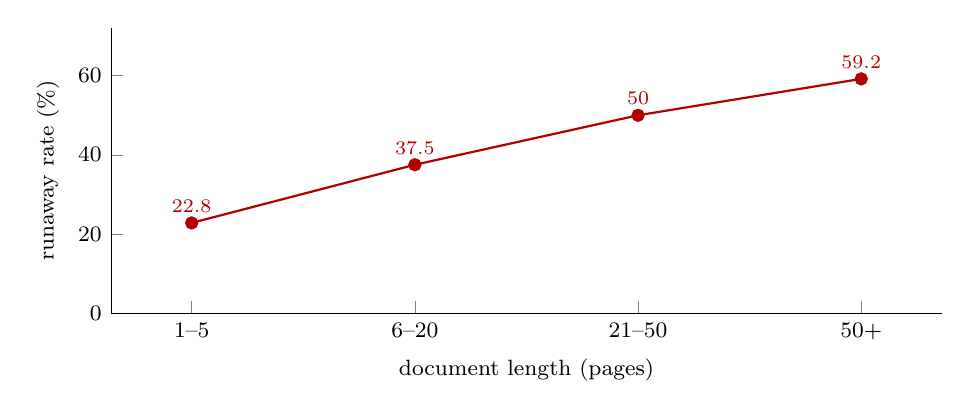
\begin{tikzpicture}
\begin{axis}[
  width=\columnwidth, height=5.2cm,
  ymin=0, ymax=72,
  ylabel={runaway rate (\%)}, ylabel style={font=\footnotesize},
  xlabel={document length (pages)}, xlabel style={font=\footnotesize},
  symbolic x coords={1--5,6--20,21--50,50+},
  xtick=data,
  tick label style={font=\footnotesize},
  enlarge x limits=0.12,
  axis x line*=bottom, axis y line*=left,
  nodes near coords, nodes near coords style={font=\scriptsize},
  every node near coord/.append style={/pgf/number format/fixed,/pgf/number format/precision=1},
]
\addplot[red!70!black,thick,mark=*] coordinates {(1--5,22.8) (6--20,37.5) (21--50,50.0) (50+,59.2)};
\end{axis}
\end{tikzpicture}
\caption{The structural ceiling on the base 4B agent: as documents get longer, the append-only trajectory more often exhausts the turn/token/time budget before submitting (\emph{runaway}). The rate is measured from how a rollout terminates, not from its answer score, so it is independent of the supervised-accuracy evaluation still being finalized. Per-document runaway rate correlates with page count at Pearson $r \approx 0.70$ ($n{=}25$); 38.8\% of all base-4B rollouts run away overall, reaching 100\% on the single 181-page document. The ceiling caps any training method before answer quality enters (\S\ref{sec:prelim}).}
\label{fig:runaway}
\end{figure}